% --------------------------------------------------------------- CONFIGURATIONS
\documentclass[a4paper,12pt,final,oneside]{book}
\usepackage{rapport}


% -------------------------------------------------------------- META: CONSTANTS
\newcommand{\reporttitle}{ERP}
\newcommand{\enseignants}{Youssef~\textsc{Amghar}\\ Anne~\textsc{Legait}\\ Pierre-Alain~\textsc{Millet}\\ Mohamed~\textsc{Ouhalima}}
\newcommand{\reportauthor}{Guillaume~\textsc{Abadie}\\ Thierry~\textsc{Cantenot}\\ Marina~\textsc{Julien}\\ Ahmed~\textsc{Kachkach}\\ Martin~\textsc{Wetterwald}\\ Valentina~\textsc{Zantedeschi}}
\newcommand{\hexanome}{SpecIFic}
\newcommand{\reportsubject}{Livrable de projet}
\newcommand{\stagetopic}{Dossier d'expression des besoins}
\newcommand{\dateperiod}{du 17 décembre 2013 au 11 mars 2014}
\newcommand{\HRule}{\rule{\linewidth}{0.5mm}}
\setlength{\parskip}{1ex} % Espace entre les paragraphes

\hypersetup{
	pdftitle={\reporttitle},%
		pdfauthor={\reportauthor},%
		pdfsubject={\reportsubject},%
		pdfkeywords={INSA Lyon}
}

\title{\reporttitle}
\author{\reportauthor}
%\setcounter{tocdepth}{4}


% ------------------------------------------------------------------------- FILE
\begin{document}


    % ------------------------------------------------------------------- HEADER
	\renewcommand{\chaptername}{} %\renewcommand{\thechapter}{}
	\renewcommand{\contentsname}{Sommaire}

	\pagestyle{empty}
	\pagenumbering{Roman}


    % ------------------------------------------------------------ HEADER: TITLE
	% Inspiré de http://en.wikibooks.org/wiki/LaTeX/Title_Creation
\begin{center}
	\begin{minipage}[t]{0.48\textwidth}
	  \begin{flushleft}
	    
\includegraphics [width=40mm]{images/logo_INSA.png} \\[0.5cm]
			INSA Lyon\\
			20, avenue Albert Einstein\\
			69621 Villeurbanne Cedex
	  \end{flushleft}
	\end{minipage}
	\begin{minipage}[t]{0.48\textwidth}
	  \begin{flushright}
	    %\includegraphics [width=60mm]{images/logo_Passau.jpg} \\[0.5cm]
	    %Universität Passau\\
		%Innstraße, 3\\
		%	D-94032 Passau
	  \end{flushright}
	\end{minipage} \\[2cm]

	\textsc{\Large \reportsubject}\\[0.3cm]
	\HRule \\[0.4cm]
	{\Huge \bfseries \reporttitle}\\[0.3cm]
	{\LARGE \bfseries «~\stagetopic~»}\\[0.3cm]
	{\Large \dateperiod}\\[0.4cm]
	\HRule \\[1cm]

	
\includegraphics [scale=0.35]{images/i7.jpg} \\[0.7cm]
	\begin{minipage}[t]{0.4\textwidth}
	  \begin{flushleft} \large
	    \emph{Hexanôme \textbf{\hexanome}~:}\\
	    \small \reportauthor
	  \end{flushleft}
	\end{minipage}
	\begin{minipage}[t]{0.5\textwidth}
	  \begin{flushright} \large
	    \emph{Enseignants~:} \\
	    \enseignants
	  \end{flushright}
	\end{minipage}

	\vfill
	\footnotesize{Année scolaire 2013-2014}
\end{center}


    % --------------------------------------------------- HEADER: CONFIGURATIONS
	\sloppy          % Justification moins stricte : des mots ne dépasseront pas des paragraphes

    \frontmatter
		\pagestyle{empty}
		\tableofcontents
		\addtocontents{toc}{\protect\thispagestyle{empty}}

	\mainmatter
	\pagestyle{headings}

	\renewcommand{\thechapter}{\Alph{chapter}}
	\renewcommand{\chaptermark}[1]{\markboth{\MakeUppercase{\chaptername\ \thechapter.\ #1}}{}}
	\renewcommand{\sectionmark}[1]{\markright{\thesection{} #1}}


    % ------------------------------------------------------------------ CONTENT
        \chapter{Analyse de l’existant}

\section{Existant Organisationnel}
\subsection{Structure organisationnelle de SPIE}

\section{Processus stratégiques}

Le processus de gestion de contrats de maintenance et services est divis\'e en sept sous-processus.

\begin{itemize}
    \item Offre et revue d'offre
    \item Commande et revue de commande
    \item Lancements des prestation de service et travaux
    \item R\'ealisation de prestations de maintenances
    \item R\'ealisation travaux induits
    \item Evolution du contrat
    \item Solde de l'affaire et du contrat
\end{itemize}

\subsection{Offre et revue d'offre}

Le sous-processus Offre et revue d'offre se divise en etapes majeurs~:

\begin{itemize}
    \item On commance tout d'abort l'etudie des contrat potentiel a partir de processus commercial,
    processus tarvaux ou appel d'offre. Avant la prise de decision quand a la poursuite ou non,
    il est necessaire de recuperer l'ensemble des informations. Le processus peut s'arreter ici
    en cas d'abandon.
    \item Une reponse (d'une appel d'offre par exemple) est fournie au client potentiel simplement
    pour bute que SPIE entre officielement dans la course \'a une proposition d'une solution. Alors
    commence l'etude du chiffrage, choix et validation de la solution qui sera propos\'e au client.
    \item Ensuite, l'offre initiale est r\'ealiser en interne a partir de la solution choisie, puis
    valid\'e sous la responsabilit\'e du Pilote de l'Offre.
    \item Enfin cette offre initiale est envoy\'ee au client avec courrier d'accompagnement dans les
    Delais impartie.
\end{itemize}

\subsection{Commande et revue de commande}

Le sous-processus Commande et revue de commande est l'etape comporte l'etape importante de negociation
avec le client et se divise en etapes majeurs~:

\begin{itemize}
    \item L'offre est donc envoy\'ee au client, celle ci est alors enregistr\'e, diffus\'e puis le
    porteur attritr\'e est design\'e par le Responsable Activit\'e.
    \item Ensuite, pour pr\'epar\'e la negociation avec le client, arrive la commission de revue de
    commande puis validation des ecarts de negociation, plan d'action de validation.
    \item N\'egociation avec le client.
    \item Acceptation ou refus de la commande d\'efinitive tout juste n\'egoci\'ee avec le client.
    En cas de refus, le processus est alors abandonn\'e.
    \item Redaction et signature du contrat entre SPIE et le client.
\end{itemize}

\subsection{Lancements des prestation de service et travaux}

Le sous-processes Lancements des prestation de service et travaux se divise en etapes majeurs~:

\begin{itemize}
    \item Prise en compte du dossier contractuel et du dossier d'etude par le Responsable d'Affaire.
    \item Realisation du dossier complet et analyse r\'ealis\'ee.
    \item Hello
\end{itemize}

\subsection{R\'ealisation de prestations de maintenances}

Le sous-processes Lancements des prestation de service et travaux se divise en etapes majeurs~:

\begin{itemize}
    \item Hello
\end{itemize}

\subsection{R\'ealisation travaux induits}

\begin{itemize}
    \item Hello
\end{itemize}

\subsection{Evolution du contrat}

\begin{itemize}
    \item Hello
\end{itemize}

\subsection{Solde de l'affaire et du contrat}

\begin{itemize}
    \item Hello
\end{itemize}

\section{Existant informatique}

\section{Dysfonctionnements}


        \chapter{Normes et benchmarking}


\section{Introduction}
    	Le Benchmarking a pour but d'optimiser une ou plusieurs fonctions de l'entreprise. Pour cela nous allons analyser les contextes métier et technique de ses principaux concurrents, réputés comme étant les meilleurs, ou leader dans un domaine commun à SPIE. Il faut se rapprocher de ce qui semble le plus parfait à l'heure actuelle.
    	Les buts de cette étude sont~:
    \begin{itemize}
    	\item la compréhension de leurs méthodes~;
    	\item la mise en place d'indicateurs (quantité, délais, coûts)~;
    	\item des chiffres de références pour se situer par rapport à leurs performances~;
    	\item une inspiration pour créer de meilleures pratiques à partir des leurs.
    \end{itemize}
    \bigbreak
    	Grâce à toutes ces connaissances, le benchmarking va nous permettre de~:
    \begin{itemize}
    	\item de mettre en place de meilleures pratiques (Best-practices)~;
    	\item de créer des activités et processus types~;
    	\item de pouvoir étudier l'évolution de l'entreprise grâce aux chiffres des performances des concurrents.
    \end{itemize}
    \bigbreak
    	Dans un premier temps, nous allons donc détailler quelques entreprises leader dans les domaines communs à SPIE. Puis nous nous intéresserons aux systèmes informatiques disponibles sur le marché, ainsi que ceux utilisés par les concurrents.

\section{Les concurrents, leaders du marché}
    \subsection{Présentation rapide de SPIE}
    	Leader européen dans les domaines de l'énergie et des communications, SPIE accompagne ses clients privés et publics dans la conception, la réalisation, l'exploitation et la maintenance d'installations plus économes en énergie et plus respectueuses de l'environnement.
    	Sa mission : Apporter du changement, un progrès durable et une amélioration de la qualité du cadre de vie.
    \newpage
    	Pour cela, le Groupe accompagne les collectivités et les entreprises dans la conception, la réalisation, l'exploitation et la maintenance de leurs installations, grâce à son expertise dans les domaines tels que :
    \begin{itemize}
    	\item Génie électrique
    	\item Génie mécanique
    	\item Génie climatique
    	\item Pétrole et gaz
    	\item Nucléaire
    	\item Energies renouvelables
    	\item Systèmes de communication et infogérance
    	\item Réseaux extérieurs et éclairage public
    \end{itemize}
    \bigbreak
    Chiffres clés 2012 :
    \begin{itemize}
    	\item 30 200 collaborateurs
    	\item 31 pays
    	\item 500 implantations
    	\item 4 217 millions d'euros de chiffres d'affaires (+ 4,3\%), répartis entre ses 4 segments stratégiques ("Energies" (26\%), "E-fficient building" (32\%), "Smart city" (25\%) et "Industry services" (17\%)).
    \end{itemize}

    \subsection{Les concurrents en général}
    Vinci Energies (Siège social en France ; Chiffre d'affaire de 9 milliards d’euros en 2012)
    Eiffage (Siège en social en France ; Chiffre d'affaire de 14 milliards d’euros en 2012)
    	Nous allons étudier ici les best practices de deux de ces groupes : Vinci Energies et Eiffage.

    \subsection{Vinci Energies}
    	Le pôle Energies de VINCI, issu du rapprochement de VINCI Energies et de Cegelec en 2010 est leader en France et acteur majeur en Europe.
    	Expert dans chacun de ses domaines technologiques de prédilection et expert du métier de ses clients, VINCI Energies bâtit à partir de leurs besoins des offres qui répondent à leur enjeux de performance, de fiabilité et de sécurité en :
    \begin{itemize}
    	\item Energie électrique
    	\item Génie climatique et thermique
    	\item Mécanique
    	\item Technologies de l'information et de la communication
    \end{itemize}
    \bigbreak
    	Pour cela il intervient depuis l'ingénierie et la réalisation, jusqu'à la maintenance, l'exploitation et le facility management. Il intervient au service des collectivités publiques et des entreprises pour déployer, équiper, faire fonctionner et optimiser leurs infrastructures d'énergie, de transport et de communication, leurs sites industriels et leurs bâtiments.
    \newpage
    Chiffres clés 2012 :
    \begin{itemize}
    	\item 64 00 collaborateurs
    	\item 45 pays
    	\item 9 milliards d'euros de chiffres d'affaires
    \end{itemize}

    \subsection{Eiffage}
    	Leader européen des concessions et du BTP, Eiffage exerce ses activités à travers cinq métiers :
    \begin{itemize}
    	\item Concessions et partenariats public-privé (énergie, réseaux, grands ouvrages d'infrastructures autoroutières et ferroviaires...)
    	\item Construction (facily management, bâtiment, immobilier...)
    	\item Travaux publics (génie civil, route...)
    	\item Energie (génie électrique, génie climatique...)
    	\item Métal (maintenance industrielle...)
    \end{itemize}
    \bigbreak
    	Si la notoriété du groupe provient de ses réalisations de référence, son engagement pour l'environnement et la sauvegarde de la biodiversité est mis en oeuvre sur l'ensemble de ses chantiers d'infrastructures. Aménager et construire tout en valorisant la qualité de vie de chacun est bien la marque d'Eiffage.
    \bigbreak
    Chiffres clés 2012 :
    \begin{itemize}
    	\item 70 00 collaborateurs
    	\item 13 pays
    	\item 14 milliards d'euros de chiffres d'affaires
    \end{itemize}

    \subsection{Les Best-practices relevées}
    \begin{itemize}
    	\item Définir le périmètre des interventions (choisir les prestations à mettre dans le contrat, définir la gestion des délais et dates, et choisir les modalités de paiement etc).
    	\item Mesures des performances des prestations et mise en place de pénalité.
    	\item Délimitation des garanties du contrat de maintenance.
    	\item Assurer la traçabilité de l'exécution du contrat par la constitution d'une base de données de preuves.
    	\item Possibilité d'utiliser un logiciel de contrat de maintenance tel que G-CONTRATS, ou le GMAO (Gestion de Maintenance Assistée par Ordinateur) de Technic-Soft. Ils permettent des renouvellements automatiques de contrats et de facturations, de planifier les visites, de surveiller les échéances etc.
    	\item Possibilité de déléguer certaines activités de maintenance à des prestataires.
    	\item Définir le paiement de ces prestataires.
    \end{itemize}



\section{Benchmarking des ERP existants}

    Il existe un nombre considérables d'ERPs, autant commerciaux que libres, existent dans le marché. Les coûts, le processus d'intégration et les méthodes utilisées pour modéliser les process métiers variant d'un ERP à l'autre, un benchmarking critique s'imposait afin d'extraire les solutions les plus adaptées aux besoins de SPIE.

    Certains ERPs se prévalent d'une certaine généricité: adaptés aux petites comme aux grandes entreprises et à tous les secteurs et métiers. On peut citer la famille d'ERPs SAGE par exemple, qui propose des solutions généralistes. D'autres ERP comme SAP ByDesign restent adaptés à une grande variété de secteurs mais plutôt adaptés à des entreprises d'une certaine taille (PME dans le cas de ByDesign).

    Dans la suite, nous allons voir plusieurs solutions ERP et analyser leurs fonctionnalités / modèles métiers.

    \subsection{SAP}

        SAP est une multinationale, dont le siège est à Walldorf en Allemagne, qui conçoit et commercialise des logiciels de gestion et de maintenance, principalement à destination des entreprises et institutions.

        SAP a un chiffre d'affaire de 16,22 milliards € et est le plus gros concepteur de logiciels en Europe, et le 4ème à l'échelle mondiale. Tous les indicateurs montrent que l'entreprise est en bonne santé et ne risque pas de couper le support de ces logiciels.

        Le produit phare de SAP est \textit{SAP ERP}, un ERP hautement modulaire contenant un très grand nombre de modules.

        Les modules ERP rentrent dans trois catégories principales : Logistique, Gestion comptable et Ressources humaines.

        Parmi les fonctionnalités proposées :

        \begin{itemize}
            \item Facturation
            \item La gestion des achats
            \item Commandes de biens, de services
            \item Contrôle des factures
            \item Gestion des stocks
            \item Entrées, sorties, transferts de stocks
            \item Contrats, demandes d'achats, etc.
            \item Inventaire
            \item Solutions e-commerce
        \end{itemize}


        La solution SAP la mieux adaptée à SPIE est \textit{SAP Business ByDesign} : cet ERP est adapté aux PME, voir aux sociétés à taille intermédiaire (jusqu'à 5000 employés). Il est commercialisé en mode SaaS (Software as a Service).

        Une licence \textit{SAP ByDesign} coûte 130€ par utilisateur par an.

        Parmi ses points forts:

        \begin{itemize}
            \item SAP est une entreprise leader du marché, à la santé financière solide~;
            \item Étant distribué en SaaS, son déploiement est rapide et ne nécessite l'achat de serveurs et leur administration, ce qui est adapté au cas SPIE (où tout est fait pour déléguer la gestion des infrastructures techniques)~;
            \item L'étude ne portant que sur la partie maintenance d'ARIS, nous pouvons raisonnablement considérer ARIS comme une PME et a donc un dimensionnement adapté à l'utilisation d'\textit{SAP ByDesign}~;
            \item SAP ByDesign est hautement modulaire, et propose déjà des modules visant les opérations de maintenance, la facturation... ce qui diminue la charge de développement spécifique~;
            \item SAP ByDesign a un design \textit{responsive} (qui s'adapte au type de périphérique et à la taille de l'écran) et est accessible depuis le web : deux points qui en font un outil adapté pour une utilisation \textit{in situ} lors des interventions de SPIE, ce qui manque cruellement à leurs solutions actuelles~;
            \item De multiples formations SAP, adaptés à tous les types d'utilisateurs, sont disponibles gratuitement sur le web, ce qui simplifie l'auto-formation
        \end{itemize}


    \subsection{Sage}

        \textit{Sage} est une multinationale éditrice de logicielle, fondée en 1981 et basée à Newcastle.

        3ème éditeur d'ERPs en Europe (derrière \textit{Dassault Systemes} et \textit{SAP}), elle a dégagé un chiffre d'affaire de 420 millions d'euros.

        L'un des produits phares de \textit{Sage} est \textit{SAGE ERP X3 Edition} : Cette solution s'adresse particulièrement aux entreprises de taille moyenne dans les secteurs de l'industrie, de la distribution et des services.

        Sage propose de multiples solutions ``sur mesure'' : des solutions pour le BTP, des solutions pour les entreprises de service, ... Malheureusement, la multiplicité des solutions fait que peu de ressources spécifiques sont disponible pour chacun de ces ERPs.

        De plus, certains modules comme la gestion des stocks et la gestion du parc matériel ne semblent pas aussi complets que ceux proposé par d'autres solutions (comme \textit{SAP}).

        \chapter{Cibles de fonctionnement}

\section{Les attentes client}

Nous avons été contacté par la société SPIE Sud-Est afin d'améliorer certains points dans le processus de gestion des contrats de maintenance. Il s'agit de proposer des solutions pour :

\begin{itemize}
    \item le développement de procédures métier et de supports d'exploitation par les entités de maintenance et service
    \item la standardisation des procédures métier et de supports d'exploitation pour les entités exerçant le même métier sur le même secteur d'activité client
    \item l'analyse des risques propres à chaque métier sur le même secteur d'activité client
    \item l'amélioration de la définition des limites des interfaces avec les autres processus
    \item la mise en place d'un Info centre sur l'intranet
\end{itemize}

Les chapitres précédents --- analyse de l'existant et benchmarking --- permettent d'identifier les axes sur lesquels le système d'information de SPIE ne suit pas les bonnes pratiques, et où des améliorations sont à prévoir.

    Nous allons donc citer dans ce document certains thèmes d'amélioration possibles au travers des axes suivants~:

    \begin{enumerate}
        \item Réorganisation de la logique des processus existants~;
        \item Réorganisation des acteurs des processus métiers de SPIE pour suivre les ``best-practices'' dégagées~;
        \item Réorganisation des acteurs~;
        \item Réorganisation de l'architecture applicative~;
    \end{enumerate}

\section{Réorganisation des processus}

\subsection{Processus Retour d'expérience}

Un premier problème que nous avions identifié dans les processus actuels de SPIE-Sud-Est, est qu'il n'existe à l'heure actuel, aucun processus dédié aux retours que soit du client, ou des
differents intervenants sur le contrat. Pour cela, nous ajoutons donc trois nouveau processus au sous-processus \textit{Solde de l'affaire et du contrat}~:

\begin{description}
    \item[Retour d'expérience client] afin que les clients puissent s'exprimer sur leur expérience avec SPIE~;
    \item[Réunion retour d'expérience interne] afin que les différents intervenants sur le contrat puissent communiquer les bons et les mauvais points concernant le déroulement du contrat de manière interne~;
    \item[Bilan du contrat] afin de prendre en compte l'ensemble des retours récoltés lors des \textit{Retour d'expérience client} et de la \textit{Réunion retour d'expérience interne}.
\end{description}

\begin{figure}[h!]
	\centering
	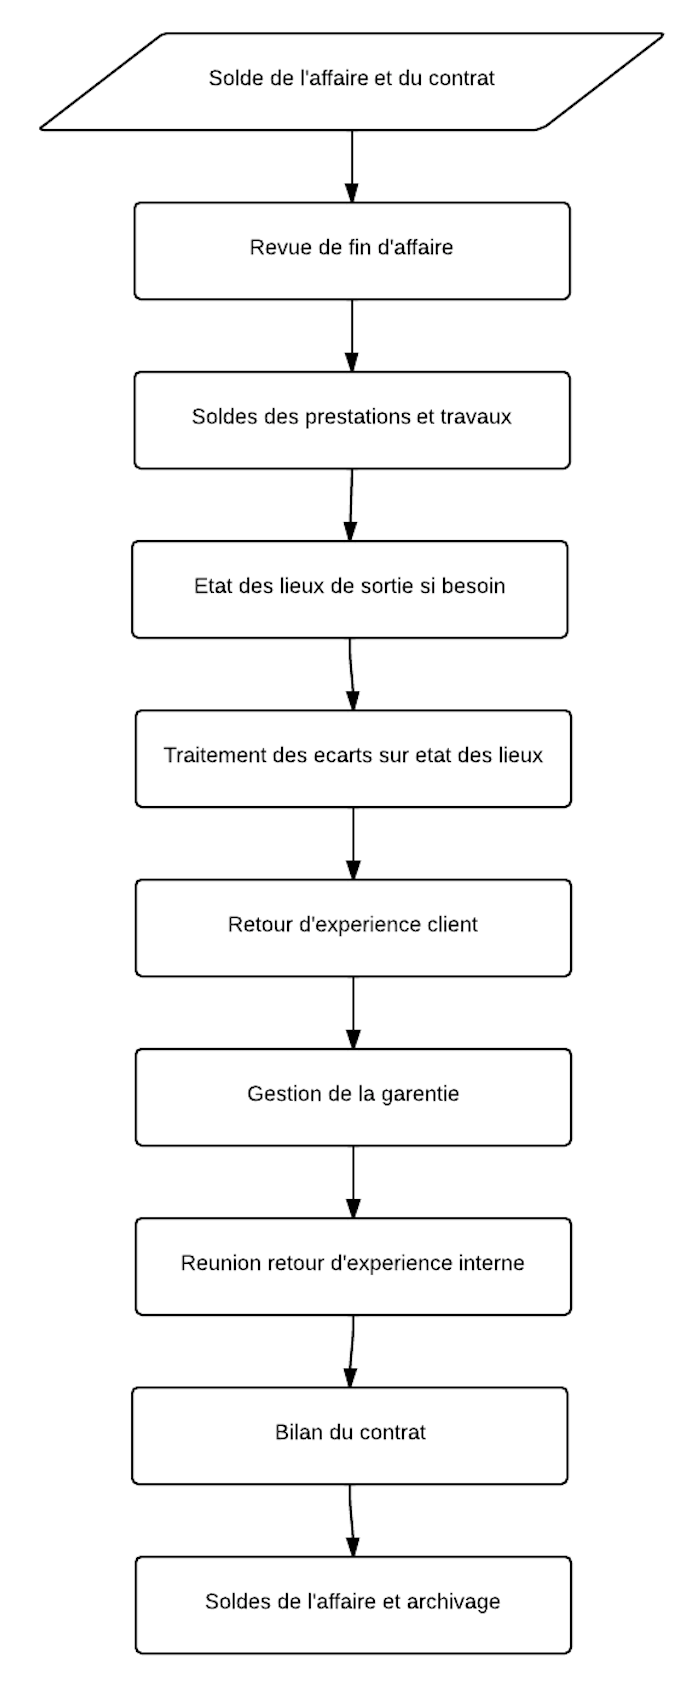
\includegraphics[width=0.45\linewidth]{images/processus_retour_experience.png}
	\caption{Sous-processus Solde de l'affaire et du contrat}
	\label{fig:processusRetourExperience}
\end{figure}


\subsection{Revue des processus}

Le second manquement que nous avions identifié dans les processus actuels de SPIE-Sud-Est, est qu'il n'y a aucun processus permettant une visibilité sur l'ensemble des processus en cours ou terminés.
C'est pourquoi nous proposons de créer un nouveau processus indépendant et parallèle aux autres, comportant deux sous-processus~:

\begin{description}
    \item[Revues des processus soldés] uniquement dédié aux processus soldés depuis la dernière revue, et qui permet de centraliser les retours sur les processus \textit{Bilan du contrat}~;
    \item[Revues des processus en cours] quant à lui est dédié aux processus en cours, afin de leur affecter les ressources matérielles et humaines nécessaires.
\end{description}

\begin{figure}[h!]
	\centering
	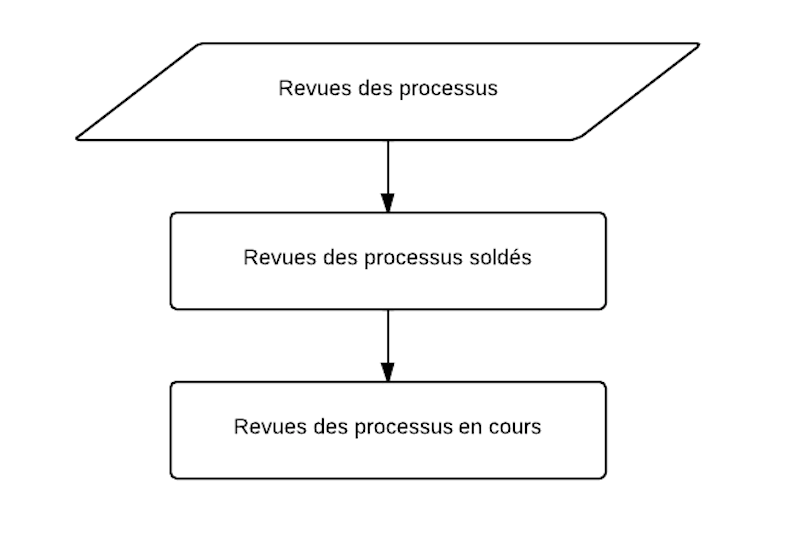
\includegraphics[width=0.45\linewidth]{images/processus_revues.png}
	\caption{Nouveau processus de revues}
	\label{fig:processusRevue}
\end{figure}

\begin{figure}[h!]
	\centering
	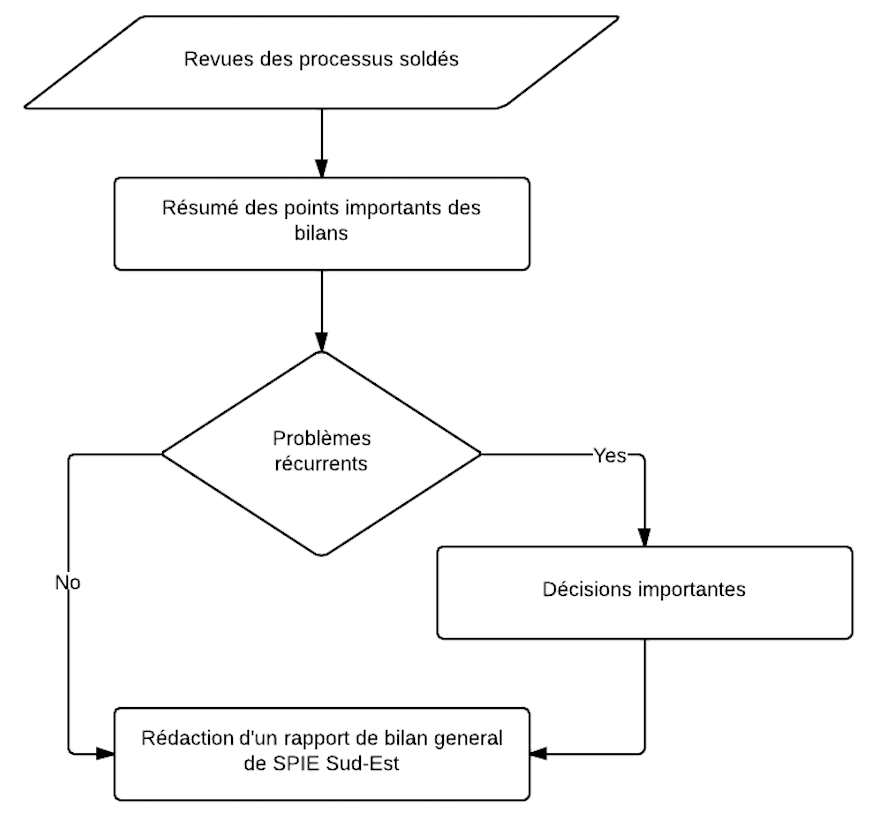
\includegraphics[width=0.45\linewidth]{images/processus_revues_solde.png}
	\caption{Nouveau processus de revues sold\'e}
	\label{fig:processusRevueSolde}
\end{figure}

\begin{figure}[h!]
	\centering
	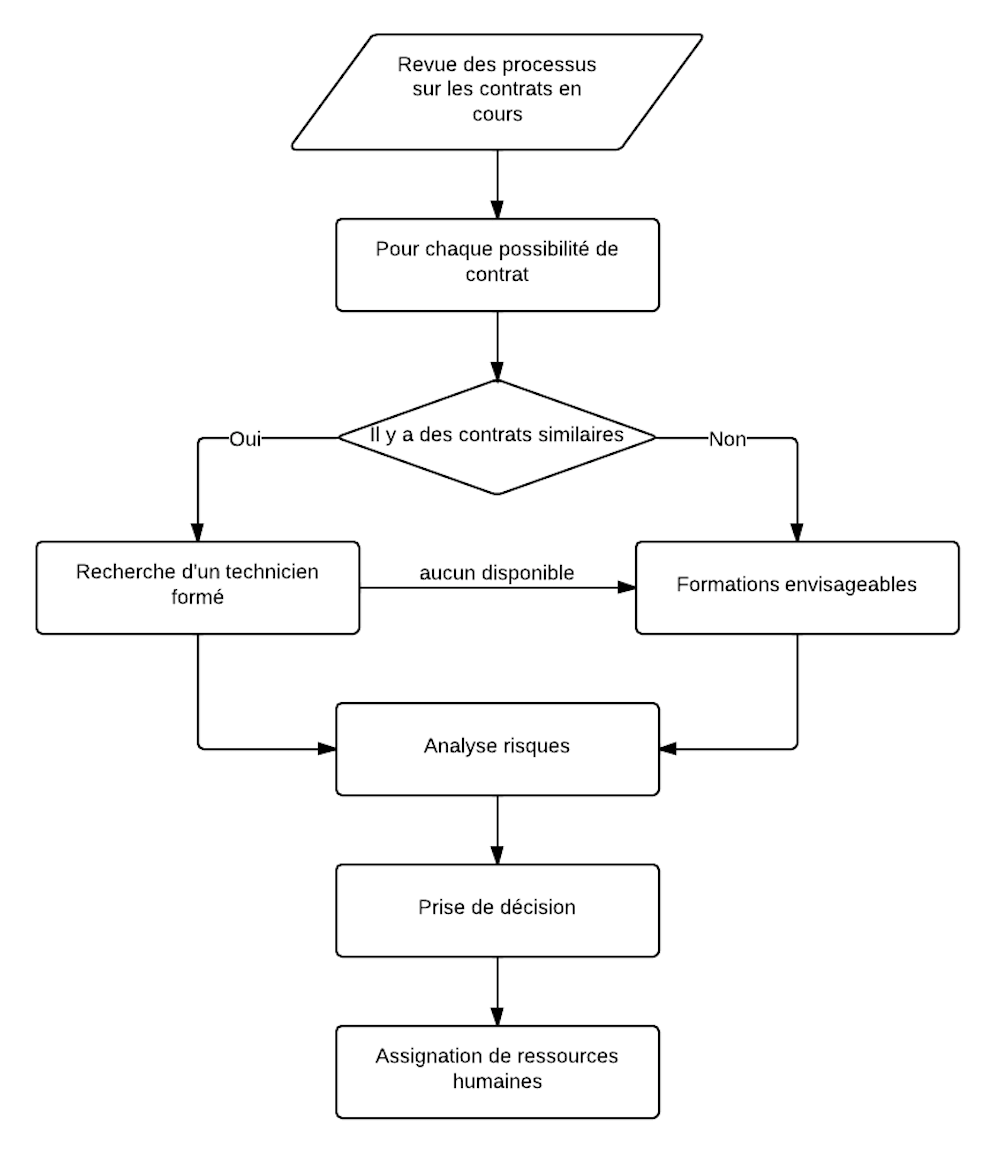
\includegraphics[width=0.45\linewidth]{images/processus_revues_actuels.png}
	\caption{Nouveau processus de revues en cours}
	\label{fig:processusRevueCours}
\end{figure}

\section{Réorganisation des acteurs}

\section{Réorganisation de l'architecture applicative}

Nous avons retravaillé l'architecture applicative afin de prendre en compte les nouvelles technologies suivantes~:

    \begin{itemize}
        \item un CRM (Customer Relationship Management)
        \item une application mobile
        \item un moteur de recommendations
    \end{itemize}

Ces nouvelles technologies sont détaillées pour précisement dans la section \vref{progres_tech}.

\begin{figure}[h!]
	\centering
	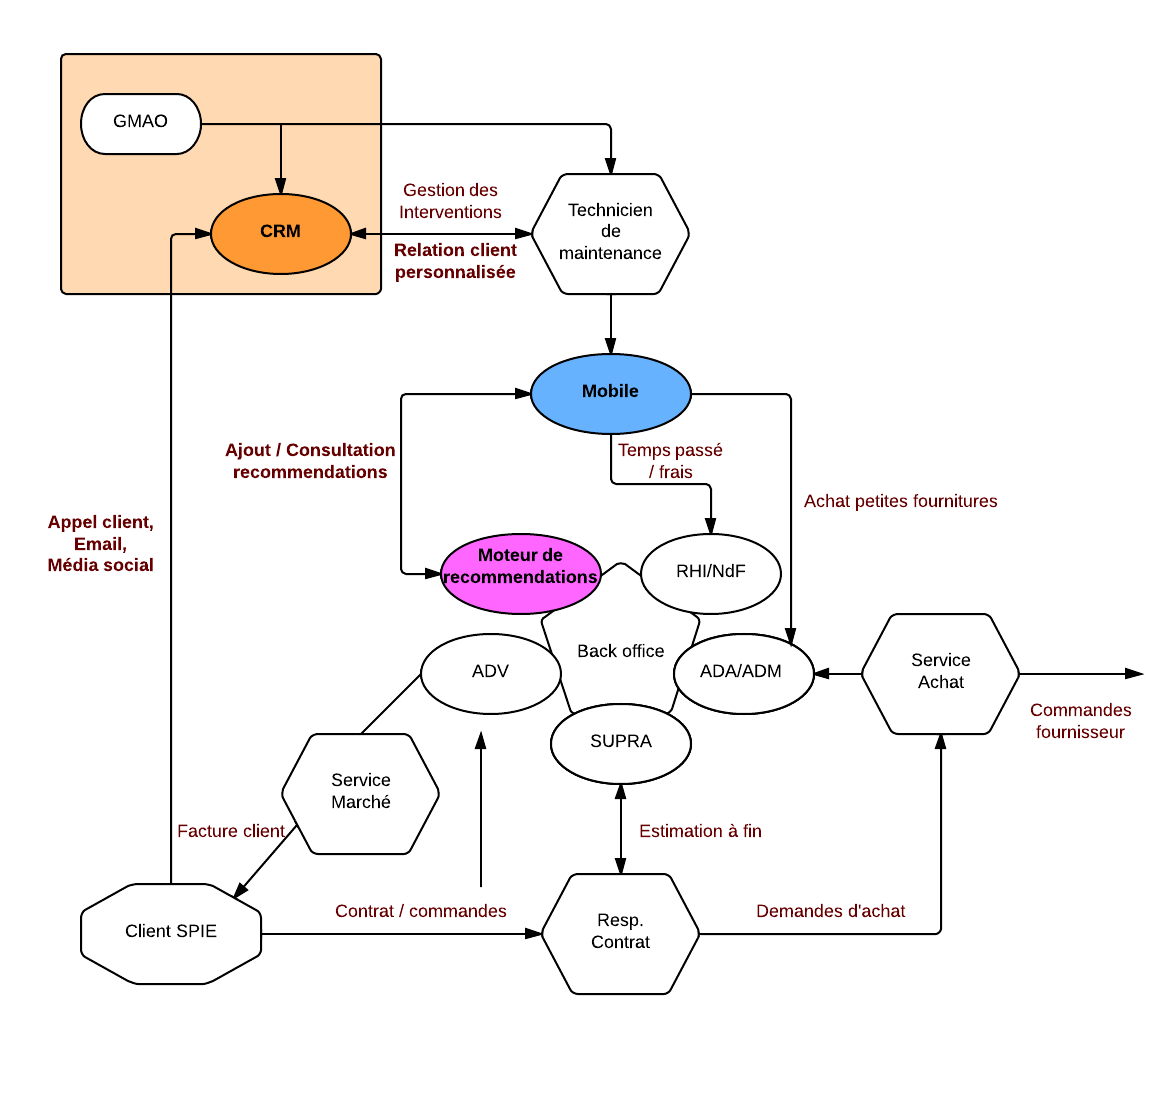
\includegraphics[width=1\linewidth]{images/cartographie_applicative_amelioree.png}
	\caption{Nouvelle architecture applicative}
	\label{fig:nouvelleArchitectureApplicative}
\end{figure}


        \chapter{Thèmes de progrès}

\section{Thèmes de progrès fonctionnels}

\section{Thèmes de progrès organisationnels}

\section{Thèmes de progrès technologiques}

    L'intégration de nouvelles technologies peut permettre à SPIE de se démarquer de la concurrence en changeant de manière radicale la gestion de certaines opérations.

    Nous allons nous intéresser à certaines technologies que SPIE pourrait intégrer~:

        \subsubsection{Gestion de la Relation Client avec un CRM}

            Quand on s'intéresse à la cartographie générale du SI de SPIE, la première chose qu'on remarque est l'absence d'une gestion de la Relation Client en utilisant un outil dédié, de type CRM.

            Les outils CRM (\textit{Customer Relationship Management}, ou Gestion de la Relation Client) permettent une gestion optimale la Relation Client avec des outils de modélisation, de reporting et de prédiction.

            L'utilisation d'outils dédiés permet autant d'améliorer les processus de Relation Client que de prédire les attentes de clients et ainsi prévenir les échecs et mieux s'y préparer. Là où SPIE utilise actuellement plusieurs outils (\textit{Clarify}, \textit{ADV}, \textit{SUPRA}) aux infrastructures parfois séparées, l'utilisation d'un seul CRM simplifierai les processus de facturation, de suivi contrats et autres processus clients, et permettrait une meilleure intégration entre ces derniers.

            Les outils CRM permettent en outre de mener des campagnes de prospection, de suivre les opportunités commerciales et de fidéliser les clients.

            On peut citer à titre d'exemple \textit{Salesforce}, l'un des leaders du marché qui propose un CRM en mode \textit{SaaS}.

        \subsubsection{SI utilisable pendant les interventions (application mobile)}

            Les techniciens ne peuvent actuellement pas utiliser les applications SPIE pendant une intervention: ils ne disposent pas de tablettes fournies à ce but et les applications SPIE ne sont pas optimisés (ou même parfois utilisables) sur des terminaux mobiles.

            Fournir des tablettes aux techniciens et leur donner accès au système d'information de SPIE leur permettrait de proposer une meilleur service aux clients chez lesquels ils interviennent en ayant constamment sous les yeux les informations relatives à des interventions précédentes (par eux ou d'autres techniciens), et pouvant entrer au fur et à mesure des informations sur le déroulement de l'intervention afin d'assurer une meilleure réactivité et afin qu'aucune information ne soit oubliée (ce qui risque d'arriver si le technicien ne fait l'entrée de données qu'une fois l'intervention terminée).

            Il faut noter que les éditeurs d'ERPs, et plus généralement de logiciels modernes adoptent souvent aujourd'hui une politique de \textit{``Mobile first''} et proposent ainsi des outils accessibles aussi bien depuis ordinateur que depuis mobile et tablettes, sans sacrifier les fonctionnalités de l'ERP ou son ergonomie. SAP ByDesign s'adapte ainsi directement au terminal utilisé pour y accéder, et l'éditeur de CRM \textit{Salesforce} propose un \textit{framework} CRM adapté pour mobile, \textit{Salesforce1}, s'intégrant avec la totalité de sa ligne de produit.


        \subsubsection{Moteur de recommandation et de préventions des risques}

            SPIE peut valoriser ses années d'expérience dans le domaine de la maintenance en créant un moteur de recommandation exploitant toutes les données récoltées lors d'interventions passées afin de proposer aux techniciens des recommandations similaires à celle qu'ils souhaitent effectuer.

            De cette manière, l'expérience des techniciens SPIE sera réellement mutualisée et mise à profit~:

            \begin{itemize}
                \item Priorisation des points à vérifier pendant l'intervention, ce qui permet d'assurer des interventions rapides et efficaces~;
                \item Prévention d'erreurs commises lors d'interventions similaires~;
                \item Possibilité de contacter facilement un technicien étant intervenu dans un cas similaire afin de faire un partage d'information.
            \end{itemize}

            Les critères à privilégier pour recommander des livraisons sont nombreux. En voici quelque uns~:
            \begin{itemize}
                \item Client visé par l'intervention~;
                \item Matériel utilisé~;
                \item Zone géographique~;
                \item ``Symptomes'' de panne~;
                \item ...
            \end{itemize}

    % TODO : donner + de nouvelles technologies et notamment parler de ça :
    %
    % * Affecter un (ou des) techniciens à chaque client. Le technicien connaîtra déjà l'infrastructure du client à chaque intervention ce qui devrait accélérer les choses et donner un meilleur processus

    % ------------------------------------------------------------------- FOOTER
\end{document}
